% Created by tikzDevice version 0.12.6 on 2024-03-07 17:07:45
% !TEX encoding = UTF-8 Unicode
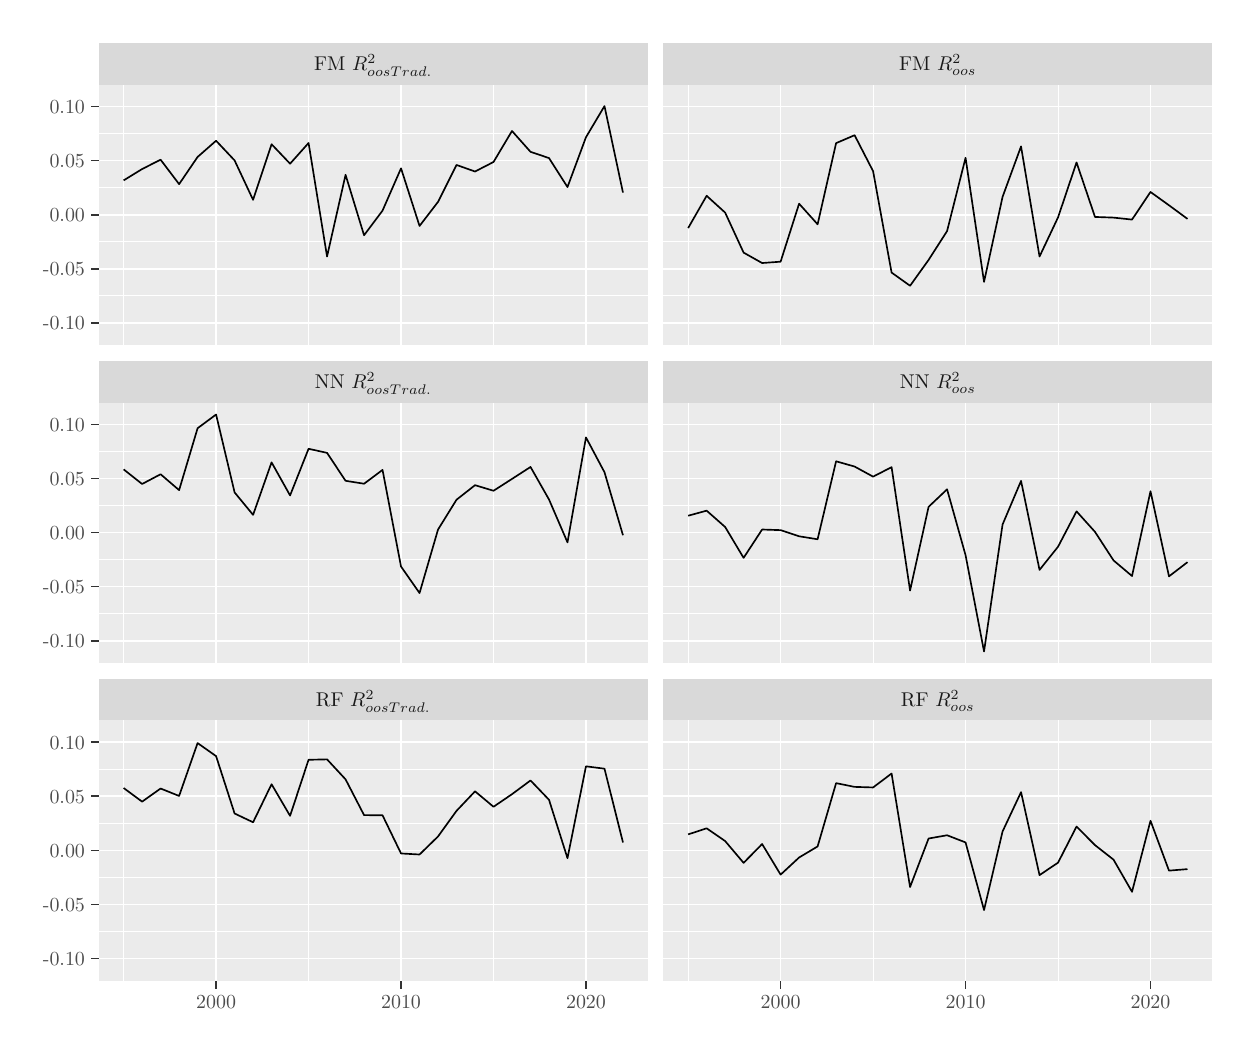
\begin{tikzpicture}[x=1pt,y=1pt]
\definecolor{fillColor}{RGB}{255,255,255}
\path[use as bounding box,fill=fillColor,fill opacity=0.00] (0,0) rectangle (433.62,361.35);
\begin{scope}
\path[clip] (  0.00,  0.00) rectangle (433.62,361.35);
\definecolor{drawColor}{RGB}{255,255,255}
\definecolor{fillColor}{RGB}{255,255,255}

\path[draw=drawColor,line width= 0.6pt,line join=round,line cap=round,fill=fillColor] (  0.00,  0.00) rectangle (433.62,361.35);
\end{scope}
\begin{scope}
\path[clip] ( 25.65,246.50) rectangle (224.13,340.69);
\definecolor{fillColor}{gray}{0.92}

\path[fill=fillColor] ( 25.65,246.50) rectangle (224.13,340.69);
\definecolor{drawColor}{RGB}{255,255,255}

\path[draw=drawColor,line width= 0.3pt,line join=round] ( 25.65,264.45) --
	(224.13,264.45);

\path[draw=drawColor,line width= 0.3pt,line join=round] ( 25.65,283.99) --
	(224.13,283.99);

\path[draw=drawColor,line width= 0.3pt,line join=round] ( 25.65,303.53) --
	(224.13,303.53);

\path[draw=drawColor,line width= 0.3pt,line join=round] ( 25.65,323.07) --
	(224.13,323.07);

\path[draw=drawColor,line width= 0.3pt,line join=round] ( 34.67,246.50) --
	( 34.67,340.69);

\path[draw=drawColor,line width= 0.3pt,line join=round] (101.50,246.50) --
	(101.50,340.69);

\path[draw=drawColor,line width= 0.3pt,line join=round] (168.33,246.50) --
	(168.33,340.69);

\path[draw=drawColor,line width= 0.6pt,line join=round] ( 25.65,254.68) --
	(224.13,254.68);

\path[draw=drawColor,line width= 0.6pt,line join=round] ( 25.65,274.22) --
	(224.13,274.22);

\path[draw=drawColor,line width= 0.6pt,line join=round] ( 25.65,293.76) --
	(224.13,293.76);

\path[draw=drawColor,line width= 0.6pt,line join=round] ( 25.65,313.30) --
	(224.13,313.30);

\path[draw=drawColor,line width= 0.6pt,line join=round] ( 25.65,332.84) --
	(224.13,332.84);

\path[draw=drawColor,line width= 0.6pt,line join=round] ( 68.08,246.50) --
	( 68.08,340.69);

\path[draw=drawColor,line width= 0.6pt,line join=round] (134.91,246.50) --
	(134.91,340.69);

\path[draw=drawColor,line width= 0.6pt,line join=round] (201.74,246.50) --
	(201.74,340.69);
\definecolor{drawColor}{RGB}{0,0,0}

\path[draw=drawColor,line width= 0.6pt,line join=round] ( 34.67,306.16) --
	( 41.35,310.26) --
	( 48.03,313.64) --
	( 54.72,304.81) --
	( 61.40,314.63) --
	( 68.08,320.49) --
	( 74.77,313.38) --
	( 81.45,299.13) --
	( 88.13,319.23) --
	( 94.82,312.19) --
	(101.50,319.68) --
	(108.18,278.66) --
	(114.87,308.18) --
	(121.55,286.33) --
	(128.23,295.24) --
	(134.91,310.52) --
	(141.60,289.70) --
	(148.28,298.40) --
	(154.96,311.74) --
	(161.65,309.37) --
	(168.33,312.81) --
	(175.01,324.02) --
	(181.70,316.48) --
	(188.38,314.23) --
	(195.06,303.75) --
	(201.74,321.76) --
	(208.43,333.01) --
	(215.11,301.76);
\end{scope}
\begin{scope}
\path[clip] ( 25.65,131.66) rectangle (224.13,225.84);
\definecolor{fillColor}{gray}{0.92}

\path[fill=fillColor] ( 25.65,131.66) rectangle (224.13,225.84);
\definecolor{drawColor}{RGB}{255,255,255}

\path[draw=drawColor,line width= 0.3pt,line join=round] ( 25.65,149.60) --
	(224.13,149.60);

\path[draw=drawColor,line width= 0.3pt,line join=round] ( 25.65,169.15) --
	(224.13,169.15);

\path[draw=drawColor,line width= 0.3pt,line join=round] ( 25.65,188.69) --
	(224.13,188.69);

\path[draw=drawColor,line width= 0.3pt,line join=round] ( 25.65,208.23) --
	(224.13,208.23);

\path[draw=drawColor,line width= 0.3pt,line join=round] ( 34.67,131.66) --
	( 34.67,225.84);

\path[draw=drawColor,line width= 0.3pt,line join=round] (101.50,131.66) --
	(101.50,225.84);

\path[draw=drawColor,line width= 0.3pt,line join=round] (168.33,131.66) --
	(168.33,225.84);

\path[draw=drawColor,line width= 0.6pt,line join=round] ( 25.65,139.83) --
	(224.13,139.83);

\path[draw=drawColor,line width= 0.6pt,line join=round] ( 25.65,159.37) --
	(224.13,159.37);

\path[draw=drawColor,line width= 0.6pt,line join=round] ( 25.65,178.92) --
	(224.13,178.92);

\path[draw=drawColor,line width= 0.6pt,line join=round] ( 25.65,198.46) --
	(224.13,198.46);

\path[draw=drawColor,line width= 0.6pt,line join=round] ( 25.65,218.00) --
	(224.13,218.00);

\path[draw=drawColor,line width= 0.6pt,line join=round] ( 68.08,131.66) --
	( 68.08,225.84);

\path[draw=drawColor,line width= 0.6pt,line join=round] (134.91,131.66) --
	(134.91,225.84);

\path[draw=drawColor,line width= 0.6pt,line join=round] (201.74,131.66) --
	(201.74,225.84);
\definecolor{drawColor}{RGB}{0,0,0}

\path[draw=drawColor,line width= 0.6pt,line join=round] ( 34.67,201.74) --
	( 41.35,196.45) --
	( 48.03,199.98) --
	( 54.72,194.24) --
	( 61.40,216.60) --
	( 68.08,221.56) --
	( 74.77,193.41) --
	( 81.45,185.30) --
	( 88.13,204.27) --
	( 94.82,192.32) --
	(101.50,209.18) --
	(108.18,207.70) --
	(114.87,197.61) --
	(121.55,196.55) --
	(128.23,201.54) --
	(134.91,166.63) --
	(141.60,157.05) --
	(148.28,179.99) --
	(154.96,190.77) --
	(161.65,196.03) --
	(168.33,194.01) --
	(175.01,198.29) --
	(181.70,202.61) --
	(188.38,190.86) --
	(195.06,175.36) --
	(201.74,213.29) --
	(208.43,200.70) --
	(215.11,177.94);
\end{scope}
\begin{scope}
\path[clip] ( 25.65, 16.81) rectangle (224.13,111.00);
\definecolor{fillColor}{gray}{0.92}

\path[fill=fillColor] ( 25.65, 16.81) rectangle (224.13,111.00);
\definecolor{drawColor}{RGB}{255,255,255}

\path[draw=drawColor,line width= 0.3pt,line join=round] ( 25.65, 34.76) --
	(224.13, 34.76);

\path[draw=drawColor,line width= 0.3pt,line join=round] ( 25.65, 54.30) --
	(224.13, 54.30);

\path[draw=drawColor,line width= 0.3pt,line join=round] ( 25.65, 73.84) --
	(224.13, 73.84);

\path[draw=drawColor,line width= 0.3pt,line join=round] ( 25.65, 93.38) --
	(224.13, 93.38);

\path[draw=drawColor,line width= 0.3pt,line join=round] ( 34.67, 16.81) --
	( 34.67,111.00);

\path[draw=drawColor,line width= 0.3pt,line join=round] (101.50, 16.81) --
	(101.50,111.00);

\path[draw=drawColor,line width= 0.3pt,line join=round] (168.33, 16.81) --
	(168.33,111.00);

\path[draw=drawColor,line width= 0.6pt,line join=round] ( 25.65, 24.99) --
	(224.13, 24.99);

\path[draw=drawColor,line width= 0.6pt,line join=round] ( 25.65, 44.53) --
	(224.13, 44.53);

\path[draw=drawColor,line width= 0.6pt,line join=round] ( 25.65, 64.07) --
	(224.13, 64.07);

\path[draw=drawColor,line width= 0.6pt,line join=round] ( 25.65, 83.61) --
	(224.13, 83.61);

\path[draw=drawColor,line width= 0.6pt,line join=round] ( 25.65,103.15) --
	(224.13,103.15);

\path[draw=drawColor,line width= 0.6pt,line join=round] ( 68.08, 16.81) --
	( 68.08,111.00);

\path[draw=drawColor,line width= 0.6pt,line join=round] (134.91, 16.81) --
	(134.91,111.00);

\path[draw=drawColor,line width= 0.6pt,line join=round] (201.74, 16.81) --
	(201.74,111.00);
\definecolor{drawColor}{RGB}{0,0,0}

\path[draw=drawColor,line width= 0.6pt,line join=round] ( 34.67, 86.61) --
	( 41.35, 81.67) --
	( 48.03, 86.42) --
	( 54.72, 83.73) --
	( 61.40,102.84) --
	( 68.08, 98.12) --
	( 74.77, 77.39) --
	( 81.45, 74.22) --
	( 88.13, 87.97) --
	( 94.82, 76.54) --
	(101.50, 96.80) --
	(108.18, 96.95) --
	(114.87, 89.73) --
	(121.55, 76.81) --
	(128.23, 76.73) --
	(134.91, 62.95) --
	(141.60, 62.57) --
	(148.28, 69.09) --
	(154.96, 78.34) --
	(161.65, 85.40) --
	(168.33, 79.82) --
	(175.01, 84.37) --
	(181.70, 89.33) --
	(188.38, 82.35) --
	(195.06, 61.24) --
	(201.74, 94.44) --
	(208.43, 93.58) --
	(215.11, 66.92);
\end{scope}
\begin{scope}
\path[clip] (229.63,246.50) rectangle (428.12,340.69);
\definecolor{fillColor}{gray}{0.92}

\path[fill=fillColor] (229.63,246.50) rectangle (428.12,340.69);
\definecolor{drawColor}{RGB}{255,255,255}

\path[draw=drawColor,line width= 0.3pt,line join=round] (229.63,264.45) --
	(428.12,264.45);

\path[draw=drawColor,line width= 0.3pt,line join=round] (229.63,283.99) --
	(428.12,283.99);

\path[draw=drawColor,line width= 0.3pt,line join=round] (229.63,303.53) --
	(428.12,303.53);

\path[draw=drawColor,line width= 0.3pt,line join=round] (229.63,323.07) --
	(428.12,323.07);

\path[draw=drawColor,line width= 0.3pt,line join=round] (238.66,246.50) --
	(238.66,340.69);

\path[draw=drawColor,line width= 0.3pt,line join=round] (305.49,246.50) --
	(305.49,340.69);

\path[draw=drawColor,line width= 0.3pt,line join=round] (372.32,246.50) --
	(372.32,340.69);

\path[draw=drawColor,line width= 0.6pt,line join=round] (229.63,254.68) --
	(428.12,254.68);

\path[draw=drawColor,line width= 0.6pt,line join=round] (229.63,274.22) --
	(428.12,274.22);

\path[draw=drawColor,line width= 0.6pt,line join=round] (229.63,293.76) --
	(428.12,293.76);

\path[draw=drawColor,line width= 0.6pt,line join=round] (229.63,313.30) --
	(428.12,313.30);

\path[draw=drawColor,line width= 0.6pt,line join=round] (229.63,332.84) --
	(428.12,332.84);

\path[draw=drawColor,line width= 0.6pt,line join=round] (272.07,246.50) --
	(272.07,340.69);

\path[draw=drawColor,line width= 0.6pt,line join=round] (338.90,246.50) --
	(338.90,340.69);

\path[draw=drawColor,line width= 0.6pt,line join=round] (405.73,246.50) --
	(405.73,340.69);
\definecolor{drawColor}{RGB}{0,0,0}

\path[draw=drawColor,line width= 0.6pt,line join=round] (238.66,288.93) --
	(245.34,300.60) --
	(252.02,294.53) --
	(258.70,280.06) --
	(265.39,276.30) --
	(272.07,276.79) --
	(278.75,297.74) --
	(285.44,290.29) --
	(292.12,319.62) --
	(298.80,322.49) --
	(305.49,309.49) --
	(312.17,272.86) --
	(318.85,268.08) --
	(325.54,277.42) --
	(332.22,287.84) --
	(338.90,314.33) --
	(345.58,269.49) --
	(352.27,300.20) --
	(358.95,318.44) --
	(365.63,278.64) --
	(372.32,292.80) --
	(379.00,312.64) --
	(385.68,292.95) --
	(392.37,292.71) --
	(399.05,292.00) --
	(405.73,301.97) --
	(412.41,297.17) --
	(419.10,292.25);
\end{scope}
\begin{scope}
\path[clip] (229.63,131.66) rectangle (428.12,225.84);
\definecolor{fillColor}{gray}{0.92}

\path[fill=fillColor] (229.63,131.66) rectangle (428.12,225.84);
\definecolor{drawColor}{RGB}{255,255,255}

\path[draw=drawColor,line width= 0.3pt,line join=round] (229.63,149.60) --
	(428.12,149.60);

\path[draw=drawColor,line width= 0.3pt,line join=round] (229.63,169.15) --
	(428.12,169.15);

\path[draw=drawColor,line width= 0.3pt,line join=round] (229.63,188.69) --
	(428.12,188.69);

\path[draw=drawColor,line width= 0.3pt,line join=round] (229.63,208.23) --
	(428.12,208.23);

\path[draw=drawColor,line width= 0.3pt,line join=round] (238.66,131.66) --
	(238.66,225.84);

\path[draw=drawColor,line width= 0.3pt,line join=round] (305.49,131.66) --
	(305.49,225.84);

\path[draw=drawColor,line width= 0.3pt,line join=round] (372.32,131.66) --
	(372.32,225.84);

\path[draw=drawColor,line width= 0.6pt,line join=round] (229.63,139.83) --
	(428.12,139.83);

\path[draw=drawColor,line width= 0.6pt,line join=round] (229.63,159.37) --
	(428.12,159.37);

\path[draw=drawColor,line width= 0.6pt,line join=round] (229.63,178.92) --
	(428.12,178.92);

\path[draw=drawColor,line width= 0.6pt,line join=round] (229.63,198.46) --
	(428.12,198.46);

\path[draw=drawColor,line width= 0.6pt,line join=round] (229.63,218.00) --
	(428.12,218.00);

\path[draw=drawColor,line width= 0.6pt,line join=round] (272.07,131.66) --
	(272.07,225.84);

\path[draw=drawColor,line width= 0.6pt,line join=round] (338.90,131.66) --
	(338.90,225.84);

\path[draw=drawColor,line width= 0.6pt,line join=round] (405.73,131.66) --
	(405.73,225.84);
\definecolor{drawColor}{RGB}{0,0,0}

\path[draw=drawColor,line width= 0.6pt,line join=round] (238.66,184.99) --
	(245.34,186.82) --
	(252.02,180.93) --
	(258.70,169.77) --
	(265.39,180.01) --
	(272.07,179.78) --
	(278.75,177.56) --
	(285.44,176.48) --
	(292.12,204.66) --
	(298.80,202.76) --
	(305.49,199.11) --
	(312.17,202.54) --
	(318.85,157.96) --
	(325.54,188.20) --
	(332.22,194.53) --
	(338.90,170.74) --
	(345.58,135.94) --
	(352.27,181.81) --
	(358.95,197.57) --
	(365.63,165.42) --
	(372.32,173.79) --
	(379.00,186.57) --
	(385.68,179.15) --
	(392.37,168.84) --
	(399.05,163.20) --
	(405.73,193.84) --
	(412.41,163.08) --
	(419.10,168.21);
\end{scope}
\begin{scope}
\path[clip] (229.63, 16.81) rectangle (428.12,111.00);
\definecolor{fillColor}{gray}{0.92}

\path[fill=fillColor] (229.63, 16.81) rectangle (428.12,111.00);
\definecolor{drawColor}{RGB}{255,255,255}

\path[draw=drawColor,line width= 0.3pt,line join=round] (229.63, 34.76) --
	(428.12, 34.76);

\path[draw=drawColor,line width= 0.3pt,line join=round] (229.63, 54.30) --
	(428.12, 54.30);

\path[draw=drawColor,line width= 0.3pt,line join=round] (229.63, 73.84) --
	(428.12, 73.84);

\path[draw=drawColor,line width= 0.3pt,line join=round] (229.63, 93.38) --
	(428.12, 93.38);

\path[draw=drawColor,line width= 0.3pt,line join=round] (238.66, 16.81) --
	(238.66,111.00);

\path[draw=drawColor,line width= 0.3pt,line join=round] (305.49, 16.81) --
	(305.49,111.00);

\path[draw=drawColor,line width= 0.3pt,line join=round] (372.32, 16.81) --
	(372.32,111.00);

\path[draw=drawColor,line width= 0.6pt,line join=round] (229.63, 24.99) --
	(428.12, 24.99);

\path[draw=drawColor,line width= 0.6pt,line join=round] (229.63, 44.53) --
	(428.12, 44.53);

\path[draw=drawColor,line width= 0.6pt,line join=round] (229.63, 64.07) --
	(428.12, 64.07);

\path[draw=drawColor,line width= 0.6pt,line join=round] (229.63, 83.61) --
	(428.12, 83.61);

\path[draw=drawColor,line width= 0.6pt,line join=round] (229.63,103.15) --
	(428.12,103.15);

\path[draw=drawColor,line width= 0.6pt,line join=round] (272.07, 16.81) --
	(272.07,111.00);

\path[draw=drawColor,line width= 0.6pt,line join=round] (338.90, 16.81) --
	(338.90,111.00);

\path[draw=drawColor,line width= 0.6pt,line join=round] (405.73, 16.81) --
	(405.73,111.00);
\definecolor{drawColor}{RGB}{0,0,0}

\path[draw=drawColor,line width= 0.6pt,line join=round] (238.66, 69.84) --
	(245.34, 72.04) --
	(252.02, 67.44) --
	(258.70, 59.55) --
	(265.39, 66.36) --
	(272.07, 55.30) --
	(278.75, 61.49) --
	(285.44, 65.49) --
	(292.12, 88.36) --
	(298.80, 87.01) --
	(305.49, 86.80) --
	(312.17, 91.84) --
	(318.85, 50.82) --
	(325.54, 68.35) --
	(332.22, 69.53) --
	(338.90, 66.94) --
	(345.58, 42.51) --
	(352.27, 70.90) --
	(358.95, 85.11) --
	(365.63, 55.13) --
	(372.32, 59.63) --
	(379.00, 72.67) --
	(385.68, 65.96) --
	(392.37, 60.71) --
	(399.05, 49.10) --
	(405.73, 74.77) --
	(412.41, 56.75) --
	(419.10, 57.29);
\end{scope}
\begin{scope}
\path[clip] ( 25.65,111.00) rectangle (224.13,126.16);
\definecolor{fillColor}{gray}{0.85}

\path[fill=fillColor] ( 25.65,111.00) rectangle (224.13,126.16);
\definecolor{drawColor}{gray}{0.10}

\node[text=drawColor,anchor=base,inner sep=0pt, outer sep=0pt, scale=  0.72] at (124.89,116.10) {RF $R^2_{oos  Trad.}$};
\end{scope}
\begin{scope}
\path[clip] (229.63,111.00) rectangle (428.12,126.16);
\definecolor{fillColor}{gray}{0.85}

\path[fill=fillColor] (229.63,111.00) rectangle (428.12,126.16);
\definecolor{drawColor}{gray}{0.10}

\node[text=drawColor,anchor=base,inner sep=0pt, outer sep=0pt, scale=  0.72] at (328.88,116.10) {RF $R^2_{oos}$};
\end{scope}
\begin{scope}
\path[clip] ( 25.65,225.84) rectangle (224.13,241.00);
\definecolor{fillColor}{gray}{0.85}

\path[fill=fillColor] ( 25.65,225.84) rectangle (224.13,241.00);
\definecolor{drawColor}{gray}{0.10}

\node[text=drawColor,anchor=base,inner sep=0pt, outer sep=0pt, scale=  0.72] at (124.89,230.94) {NN $R^2_{oos  Trad.}$};
\end{scope}
\begin{scope}
\path[clip] (229.63,225.84) rectangle (428.12,241.00);
\definecolor{fillColor}{gray}{0.85}

\path[fill=fillColor] (229.63,225.84) rectangle (428.12,241.00);
\definecolor{drawColor}{gray}{0.10}

\node[text=drawColor,anchor=base,inner sep=0pt, outer sep=0pt, scale=  0.72] at (328.88,230.94) {NN $R^2_{oos}$};
\end{scope}
\begin{scope}
\path[clip] ( 25.65,340.69) rectangle (224.13,355.85);
\definecolor{fillColor}{gray}{0.85}

\path[fill=fillColor] ( 25.65,340.69) rectangle (224.13,355.85);
\definecolor{drawColor}{gray}{0.10}

\node[text=drawColor,anchor=base,inner sep=0pt, outer sep=0pt, scale=  0.72] at (124.89,345.79) {FM $R^2_{oos  Trad.}$};
\end{scope}
\begin{scope}
\path[clip] (229.63,340.69) rectangle (428.12,355.85);
\definecolor{fillColor}{gray}{0.85}

\path[fill=fillColor] (229.63,340.69) rectangle (428.12,355.85);
\definecolor{drawColor}{gray}{0.10}

\node[text=drawColor,anchor=base,inner sep=0pt, outer sep=0pt, scale=  0.72] at (328.88,345.79) {FM $R^2_{oos}$};
\end{scope}
\begin{scope}
\path[clip] (  0.00,  0.00) rectangle (433.62,361.35);
\definecolor{drawColor}{gray}{0.20}

\path[draw=drawColor,line width= 0.6pt,line join=round] ( 68.08, 14.06) --
	( 68.08, 16.81);

\path[draw=drawColor,line width= 0.6pt,line join=round] (134.91, 14.06) --
	(134.91, 16.81);

\path[draw=drawColor,line width= 0.6pt,line join=round] (201.74, 14.06) --
	(201.74, 16.81);
\end{scope}
\begin{scope}
\path[clip] (  0.00,  0.00) rectangle (433.62,361.35);
\definecolor{drawColor}{gray}{0.30}

\node[text=drawColor,anchor=base,inner sep=0pt, outer sep=0pt, scale=  0.72] at ( 68.08,  6.90) {2000};

\node[text=drawColor,anchor=base,inner sep=0pt, outer sep=0pt, scale=  0.72] at (134.91,  6.90) {2010};

\node[text=drawColor,anchor=base,inner sep=0pt, outer sep=0pt, scale=  0.72] at (201.74,  6.90) {2020};
\end{scope}
\begin{scope}
\path[clip] (  0.00,  0.00) rectangle (433.62,361.35);
\definecolor{drawColor}{gray}{0.20}

\path[draw=drawColor,line width= 0.6pt,line join=round] (272.07, 14.06) --
	(272.07, 16.81);

\path[draw=drawColor,line width= 0.6pt,line join=round] (338.90, 14.06) --
	(338.90, 16.81);

\path[draw=drawColor,line width= 0.6pt,line join=round] (405.73, 14.06) --
	(405.73, 16.81);
\end{scope}
\begin{scope}
\path[clip] (  0.00,  0.00) rectangle (433.62,361.35);
\definecolor{drawColor}{gray}{0.30}

\node[text=drawColor,anchor=base,inner sep=0pt, outer sep=0pt, scale=  0.72] at (272.07,  6.90) {2000};

\node[text=drawColor,anchor=base,inner sep=0pt, outer sep=0pt, scale=  0.72] at (338.90,  6.90) {2010};

\node[text=drawColor,anchor=base,inner sep=0pt, outer sep=0pt, scale=  0.72] at (405.73,  6.90) {2020};
\end{scope}
\begin{scope}
\path[clip] (  0.00,  0.00) rectangle (433.62,361.35);
\definecolor{drawColor}{gray}{0.30}

\node[text=drawColor,anchor=base east,inner sep=0pt, outer sep=0pt, scale=  0.72] at ( 20.70,252.20) {-0.10};

\node[text=drawColor,anchor=base east,inner sep=0pt, outer sep=0pt, scale=  0.72] at ( 20.70,271.74) {-0.05};

\node[text=drawColor,anchor=base east,inner sep=0pt, outer sep=0pt, scale=  0.72] at ( 20.70,291.28) {0.00};

\node[text=drawColor,anchor=base east,inner sep=0pt, outer sep=0pt, scale=  0.72] at ( 20.70,310.82) {0.05};

\node[text=drawColor,anchor=base east,inner sep=0pt, outer sep=0pt, scale=  0.72] at ( 20.70,330.37) {0.10};
\end{scope}
\begin{scope}
\path[clip] (  0.00,  0.00) rectangle (433.62,361.35);
\definecolor{drawColor}{gray}{0.20}

\path[draw=drawColor,line width= 0.6pt,line join=round] ( 22.90,254.68) --
	( 25.65,254.68);

\path[draw=drawColor,line width= 0.6pt,line join=round] ( 22.90,274.22) --
	( 25.65,274.22);

\path[draw=drawColor,line width= 0.6pt,line join=round] ( 22.90,293.76) --
	( 25.65,293.76);

\path[draw=drawColor,line width= 0.6pt,line join=round] ( 22.90,313.30) --
	( 25.65,313.30);

\path[draw=drawColor,line width= 0.6pt,line join=round] ( 22.90,332.84) --
	( 25.65,332.84);
\end{scope}
\begin{scope}
\path[clip] (  0.00,  0.00) rectangle (433.62,361.35);
\definecolor{drawColor}{gray}{0.30}

\node[text=drawColor,anchor=base east,inner sep=0pt, outer sep=0pt, scale=  0.72] at ( 20.70,137.35) {-0.10};

\node[text=drawColor,anchor=base east,inner sep=0pt, outer sep=0pt, scale=  0.72] at ( 20.70,156.90) {-0.05};

\node[text=drawColor,anchor=base east,inner sep=0pt, outer sep=0pt, scale=  0.72] at ( 20.70,176.44) {0.00};

\node[text=drawColor,anchor=base east,inner sep=0pt, outer sep=0pt, scale=  0.72] at ( 20.70,195.98) {0.05};

\node[text=drawColor,anchor=base east,inner sep=0pt, outer sep=0pt, scale=  0.72] at ( 20.70,215.52) {0.10};
\end{scope}
\begin{scope}
\path[clip] (  0.00,  0.00) rectangle (433.62,361.35);
\definecolor{drawColor}{gray}{0.20}

\path[draw=drawColor,line width= 0.6pt,line join=round] ( 22.90,139.83) --
	( 25.65,139.83);

\path[draw=drawColor,line width= 0.6pt,line join=round] ( 22.90,159.37) --
	( 25.65,159.37);

\path[draw=drawColor,line width= 0.6pt,line join=round] ( 22.90,178.92) --
	( 25.65,178.92);

\path[draw=drawColor,line width= 0.6pt,line join=round] ( 22.90,198.46) --
	( 25.65,198.46);

\path[draw=drawColor,line width= 0.6pt,line join=round] ( 22.90,218.00) --
	( 25.65,218.00);
\end{scope}
\begin{scope}
\path[clip] (  0.00,  0.00) rectangle (433.62,361.35);
\definecolor{drawColor}{gray}{0.30}

\node[text=drawColor,anchor=base east,inner sep=0pt, outer sep=0pt, scale=  0.72] at ( 20.70, 22.51) {-0.10};

\node[text=drawColor,anchor=base east,inner sep=0pt, outer sep=0pt, scale=  0.72] at ( 20.70, 42.05) {-0.05};

\node[text=drawColor,anchor=base east,inner sep=0pt, outer sep=0pt, scale=  0.72] at ( 20.70, 61.59) {0.00};

\node[text=drawColor,anchor=base east,inner sep=0pt, outer sep=0pt, scale=  0.72] at ( 20.70, 81.13) {0.05};

\node[text=drawColor,anchor=base east,inner sep=0pt, outer sep=0pt, scale=  0.72] at ( 20.70,100.67) {0.10};
\end{scope}
\begin{scope}
\path[clip] (  0.00,  0.00) rectangle (433.62,361.35);
\definecolor{drawColor}{gray}{0.20}

\path[draw=drawColor,line width= 0.6pt,line join=round] ( 22.90, 24.99) --
	( 25.65, 24.99);

\path[draw=drawColor,line width= 0.6pt,line join=round] ( 22.90, 44.53) --
	( 25.65, 44.53);

\path[draw=drawColor,line width= 0.6pt,line join=round] ( 22.90, 64.07) --
	( 25.65, 64.07);

\path[draw=drawColor,line width= 0.6pt,line join=round] ( 22.90, 83.61) --
	( 25.65, 83.61);

\path[draw=drawColor,line width= 0.6pt,line join=round] ( 22.90,103.15) --
	( 25.65,103.15);
\end{scope}
\end{tikzpicture}
